\documentclass{article}
\usepackage{geometry}
\geometry{margin=1in}
\usepackage{tikz}
\usepackage{amssymb}

% fleqn allows setting indent of display math
\usepackage[fleqn]{amsmath}
\setlength{\mathindent}{0pt} % Set indent
% Disable equation numbering (https://tex.stackexchange.com/a/360378)
\makeatletter
\renewcommand\tagform@[1]{}
\makeatother

% Disable numbering (https://tex.stackexchange.com/a/360378)
\makeatletter
\renewcommand\tagform@[1]{}
\makeatother

% Allow Unicode (some, e.g., © and £ at least)
% https://tex.stackexchange.com/questions/370278/is-there-any-reason-to-use-inputenc
\usepackage[utf8]{inputenc}

% Hyperlinks
\usepackage{hyperref}
\hypersetup{colorlinks=true, urlcolor=blue, linkcolor=blue}

% Prevent indentation of paragraphs
\setlength\parindent{0pt}
\setlength{\parskip}{\baselineskip}

% Allow 3 additional subsection levels
% https://tex.stackexchange.com/a/60212
\usepackage{titlesec}
\setcounter{secnumdepth}{6}
% H4 in HTML
\titleformat{\paragraph}{\normalfont\normalsize\bfseries}{\theparagraph}{1em}{}
\titlespacing*{\paragraph}{0pt}{3.25ex plus 1ex minus .2ex}{1.5ex plus .2ex}
% H5 in HTML
\titleformat{\subparagraph}{\normalfont\normalsize\bfseries}{\thesubparagraph}{1em}{}
\titlespacing*{\subparagraph}{0pt}{3.25ex plus 1ex minus .2ex}{1.5ex plus .2ex}
% H6 in HTML
\titleformat{\subsubparagraph}{\normalfont\normalsize\bfseries}{\thesubsubparagraph}{1em}{}
\titlespacing*{\subsubparagraph}{0pt}{3.25ex plus 1ex minus .2ex}{1.5ex plus .2ex}


\renewcommand{\mbox}{\text}
\newcommand{\ds}[0]{\displaystyle}
\newcommand{\ihat}[0]{\hat{\boldsymbol{\imath}}}
\newcommand{\jhat}[0]{\hat{\boldsymbol{\jmath}}}
\newcommand{\khat}[0]{\hat{\boldsymbol{k}}}
\newcommand{\xhat}[0]{\hat{\mathbf{x}}}
\newcommand{\yhat}[0]{\hat{\mathbf{y}}}
\newcommand{\zhat}[0]{\hat{\mathbf{z}}}
\newcommand{\rhat}[0]{\hat{\mathbf{r}}}
\newcommand{\bfvec}[1]{\vec{\mathbf{#1}}}
\newcommand{\bfcdot}[0]{\boldsymbol{\cdot}}

\usepackage{fancyhdr}
\pagestyle{fancy}
\lhead{Continuous Charge Distributions}
\rhead{\thepage}

\title{Continuous Charge Distributions}

\begin{document}

\section{Overview}

Previously, you found the electric field at a location in space due to one or more point charges by finding the electric field due to each charge and then vectorially summing the fields to get the total field (this is ``using superposition").

This process requires a significant amount of calculation if there are many charges. To reduce the number of calculations when charges are closely spaced, we sometimes assume they are continuously distributed; in this case, to compute the electric field, we need to evaluate an integral rather than a sum with many terms.

Section 21.5 of the textbook gives three examples for charges that are continuously distributed:

\begin{enumerate}

  \item charges uniformly distributed along a straight line,

  \item charges uniformly distributed on a circle, and

  \item charges uniformly distributed on a disk.

\end{enumerate}

If you read the textbook examples and the lecture notes, you should be able to identify the following steps (not necessarily in this order).

\begin{enumerate}

  \item Identify answer features

  \item Find $d\bfvec{E}$ (or $dE$ and its direction) for a $dQ$ on the charged object

  \item Find $dQ$ in terms of coordinates (e.g., $dx$, $dy$, $r$, $d\theta$, etc.)

  \item Simplify $d\bfvec{E}$ (if possible) using symmetry arguments

  \item Integrate $d\bfvec{E}$

  \item Check answer features

\end{enumerate}

In this activity, you will explicitly address all of these steps for charges that are uniformly and continuously distributed along a straight line.

\section{Finite Line of Charge}

The following diagram shows a differential charge $dQ$ at a location on the $x$--axis. Recall that the general equation for the electric field due to a point charge (with $q$ replaced with $dQ$ and $\bfvec{E}$ replaced with $d\bfvec{E}$) is

$\displaystyle d\mathbf{E} =k\frac{dQ}{r^2}\hat{\mathbf{r}}$, which has magnitude $\displaystyle dE = k\frac{dQ}{r^2}$

(In a previous activity, you found the components of $\bfvec{E}$ using two methods that are used in the textbook. You may use either method for this problem.)



\tikzset{every picture/.style={line width=0.75pt}} %set default line width to 0.75pt        

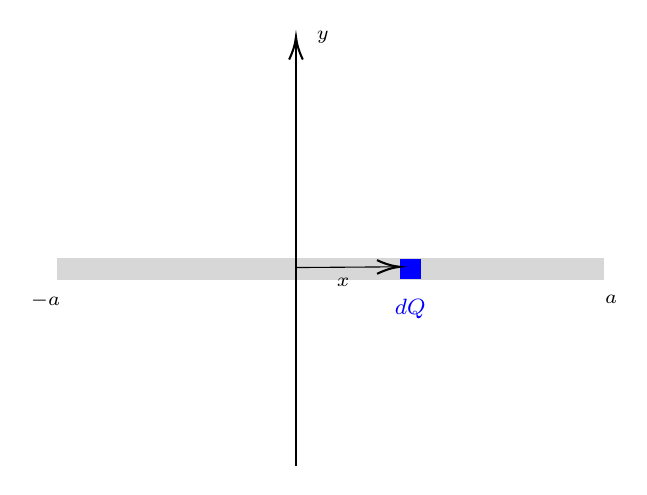
\begin{tikzpicture}[x=0.75pt,y=0.75pt,yscale=-1,xscale=1]
%uncomment if require: \path (0,229); %set diagram left start at 0, and has height of 229

%Shape: Rectangle [id:dp08213900538372076] 
\draw  [color={rgb, 255:red, 215; green, 215; blue, 215 }  ,draw opacity=1 ][fill={rgb, 255:red, 215; green, 215; blue, 215 }  ,fill opacity=1 ] (24.96,120) -- (288,120) -- (288,130) -- (24.96,130) -- cycle ;
%Straight Lines [id:da5910959185464446] 
\draw [color={rgb, 255:red, 0; green, 0; blue, 0 }  ,draw opacity=1 ]   (140,220) -- (140,15.19) ;
\draw [shift={(140,13.19)}, rotate = 90] [color={rgb, 255:red, 0; green, 0; blue, 0 }  ,draw opacity=1 ][line width=0.75]    (10.93,-3.29) .. controls (6.95,-1.4) and (3.31,-0.3) .. (0,0) .. controls (3.31,0.3) and (6.95,1.4) .. (10.93,3.29)   ;
%Shape: Rectangle [id:dp6718865848770532] 
\draw  [draw opacity=0][fill={rgb, 255:red, 0; green, 0; blue, 255 }  ,fill opacity=1 ] (200,120) -- (190,120) -- (190,130) -- (200,130) -- cycle ;
%Straight Lines [id:da8743643813694808] 
\draw [color={rgb, 255:red, 0; green, 0; blue, 0 }  ,draw opacity=1 ]   (140.09,124.35) -- (188,124.01) ;
\draw [shift={(190,124)}, rotate = 179.6] [color={rgb, 255:red, 0; green, 0; blue, 0 }  ,draw opacity=1 ][line width=0.75]    (10.93,-3.29) .. controls (6.95,-1.4) and (3.31,-0.3) .. (0,0) .. controls (3.31,0.3) and (6.95,1.4) .. (10.93,3.29)   ;

% Text Node
\draw (148.79,9.05) node [anchor=north west][inner sep=0.75pt]  [font=\scriptsize]  {$y$};
% Text Node
\draw (11,135.63) node [anchor=north west][inner sep=0.75pt]  [font=\scriptsize]  {$-a$};
% Text Node
\draw (287.64,136.23) node [anchor=north west][inner sep=0.75pt]  [font=\scriptsize]  {$a$};
% Text Node
\draw (158.48,128.4) node [anchor=north west][inner sep=0.75pt]  [font=\scriptsize]  {$x$};
% Text Node
\draw (186.41,138.49) node [anchor=north west][inner sep=0.75pt]  [font=\footnotesize]  {$\textcolor[rgb]{0,0,1}{dQ}$};


\end{tikzpicture}


\begin{enumerate}

  \item Draw the expected directions of $dE_x$ and $dE_y$ at a location on the $+y$--axis on the diagram given the location of $dQ$ shown on the figure (assume $dQ$ is positive).

  \item In the diagram, the differential charge is at a positive $x$. At the same location on the $+y$--axis, draw the expected direction of $dE_x$ and $dE_y$ on the diagram with dotted lines if $dQ$ is at $-x$.

  \item Draw the expected direction of $dE_x$ and $dE_y$ on the diagram at a location on the $-y$--axis for $dQ$ at the position in the figure.

  \item Find equations for the electric field components $dE_x$ and $dE_y$ at any location on the $y$--axis in terms of $dQ$, $x$, $y$, and $k$.

\end{enumerate}

\vskip 96.36pt

\begin{enumerate}

  \item[5.] Do your equations for $dE_x$ and $dE_y$ give the directions predicted by your answers to 1.--3.? Try plugging in values of $y=\pm a$ and $x=\pm a$.

\end{enumerate}

\vskip 36.135pt

\begin{enumerate}

  \item[6.] If the differential charge $dQ$ is at $x=0$, do you expect $dE_x$ or $dE_y$ to be zero? Is your answer consistent with the result of plugging in $x=0$ into your equations for $dE_x$ and $dE_y$?

\end{enumerate}

\vskip 12.045pt

If the charge per unit length on the line is $\lambda$, then we can write $dQ=\lambda dx$. To find $E_x$ and $E_y$, integrate $dE_x$ and $dE_y$ from $x=-a$ to $a$.

\begin{enumerate}

  \item[7.] Write down the integrals that must be evaluated to find $E_x$ and $E_y$. Do you expect either of the integrals to be zero?

\end{enumerate}

\begin{enumerate}

  \item[8.] From an integral table (or using trig substitutions), we know $\displaystyle \int \frac{du}{(u^2+a^2)^{3/2}} = \frac{u}{a^2\sqrt{u^2+a^2}} + C$. Use this to find $E_y$.

\end{enumerate}

\vskip 72.27pt

\begin{enumerate}

  \item[9.] If $y$ is negative (for example $y=-a$), is $E_y$ positive or negative? Is this consistent with your answer to 3.?

\end{enumerate}

\vskip 36.135pt

\begin{enumerate}

  \item[10.] The total charge on the line is $Q=2a\lambda$ (length $\times$ charge/length). Suppose $y\gg a$ so that you can replace $a^2+y^2$ with $y^2$. Is your equation for $E_y$ consistent with the electric field for a point charge $Q=2a\lambda$ at the origin?

\end{enumerate}

\vskip 36.135pt

\section{Long Line of Charge}

Using the result of the previous problem, we can find $E_y$ when $a \gg y$, which corresponds to a long line of charge. The result is

\begin{equation}
  E_y=\frac{2\lambda k}{y}
\end{equation}

This equation can be written more generally as

\begin{equation}
  E=\frac{2\lambda k}{r}
\end{equation}

where $r$ is the perpendicular distance from the line and the direction of $E$ is perpendicular the line with a direction that depends on the sign of the charge density $\lambda$.

A long line of charge lies along the line $y=b$.

\begin{enumerate}

  \item Find the electric field magnitude and direction at the origin.

\end{enumerate}

\vskip 72.27pt

\begin{enumerate}

  \item[2.] Find the electric field magnitude and direction at $(x,y)=(b,0)$.

\end{enumerate}

\end{document}